Generally graphing is done using the packages \texttt{tikz} and \texttt{pgfplots} inside of the \texttt{tikzpicture} environment.
Generally figures require captions and you may need to refer to them, therefore we wrap \texttt{tikzpicture} with the usual \texttt{figure} environment.

The objective here is to read through the code below before seeing the results, and see if you know what to expect.
The \texttt{pgfplots} package is extremely well documented with hundreds of examples, and very well structured tutorials.
Take the examples highlighted here as graphs we do often, but it is highly recommended to skim through the documentation \href{https://mirror.ox.ac.uk/sites/ctan.org/graphics/pgf/contrib/pgfplots/doc/pgfplots.pdf}{here}.

\begin{figure}[h]\centering
\begin{minipage}{0.45\textwidth}
    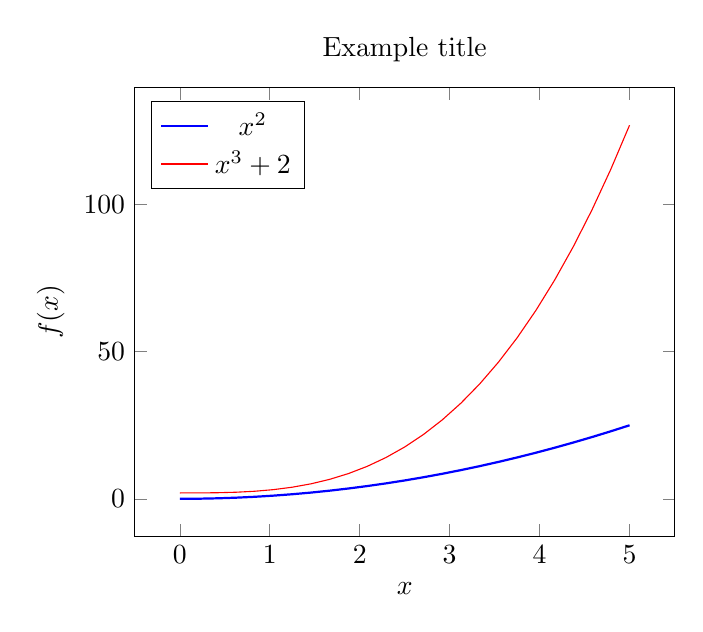
\begin{tikzpicture}
        \begin{axis} [
            xlabel=\(x\) , ylabel=\(f(x)\), title=Example title,
            domain=0:5, legend pos = north west,
        ]
            \addplot[blue, thick] {x^2};
            \addlegendentry{\(x^2\)}
            \addplot[red] {x^3+2};
            \addlegendentry{\(x^3+2\)}
        \end{axis}
    \end{tikzpicture}
    \caption{Example caption}
\end{minipage}
\hfill
\begin{minipage}{0.45\textwidth}
\begin{lstlisting}
\begin{figure}[h]\centering
    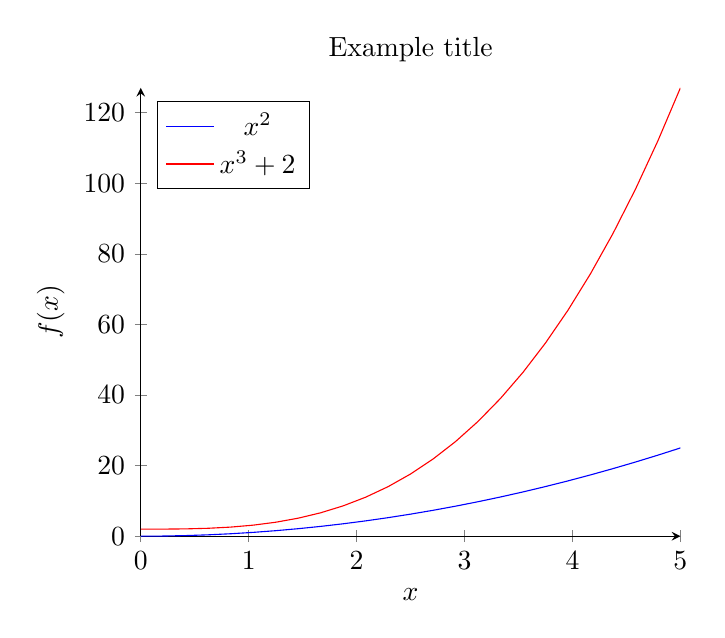
\begin{tikzpicture}
        \begin{axis} [
            xlabel=\(x\) , ylabel=\(f(x)\), title=Example title,
            domain=0:5, legend pos = north west,
            axis lines = left,
        ]
            \addplot[blue] {x^2};
            \addlegendentry{\(x^2\)}
            \addplot[red] {x^3+2}; 
            \addlegendentry{\(x^3+2\)}
        \end{axis}
    \end{tikzpicture}
    \caption{Example caption}
    \end{figure}  
\end{lstlisting}
\end{minipage}
\end{figure}

\texttt{axis} is the most common axis environment, but we can also use \texttt{semilog\underline{x}axis}, \texttt{semilog\underline{y}axis} and \texttt{loglogaxis} for our logarithmic axis needs, \texttt{polaraxis}, and more.
There are hundreds of options with names that tend to be self-evident, and the best approach is to search for examples and modify them to your needs.
\begin{lstlisting}
    \begin{axis}[
        %options here separate by commas,
    ]
        %plots here separated by colons;
    \end{axis}
\end{lstlisting} 

Plotting a function is simply a matter of using \verb|\addplot[options] {function};|.
The options include things like colour, thickness, the domain for that specific plot and much more.
Generally you will want to have the domain defined in the \texttt{axis} environment, not for each plot, but you will see plenty of examples where you do both.

We created legends by using \verb|\addlegendentry{}|, but we also have the option of using \verb|\legend{}| and describing them all in one place, as will be seen in the next example.

We have a lot of freedom with the frequency of the label ticks, whether you want them replaced with text, minimum and maximum displayed values.
Changing the options of our plot to the following, and adding a dashed-line plot gives us the graph seen below.
\begin{figure}[h]
\centering
\begin{minipage}{0.45\textwidth}
    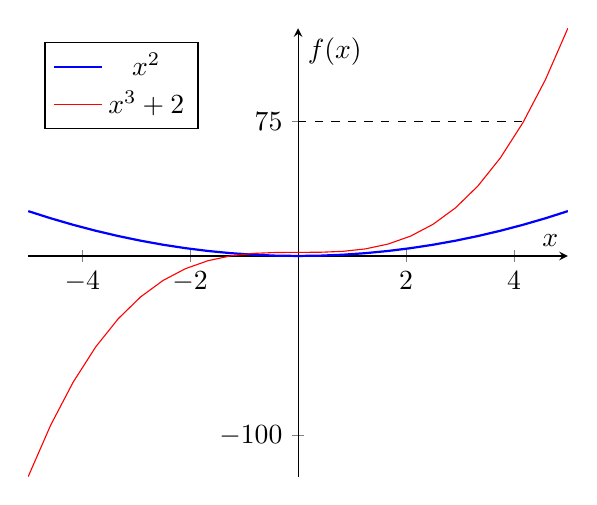
\begin{tikzpicture}
        \begin{axis} [
            xlabel=\(x\), ylabel=\(f(x)\),
            legend pos = north west,
            domain=-5:5, axis lines = center,
            ytick={-100,0,75}, 
        ]
            \addplot[blue, thick] {x^2};
            \addlegendentry{\(x^2\)}
            \addplot[red] {x^3+2};
            \addlegendentry{\(x^3+2\)}
            \addplot[dashed, domain=0:4.18] {75};
        \end{axis}
    \end{tikzpicture}    
\end{minipage}
\hfill
\begin{minipage}{0.45\textwidth}
\begin{lstlisting}
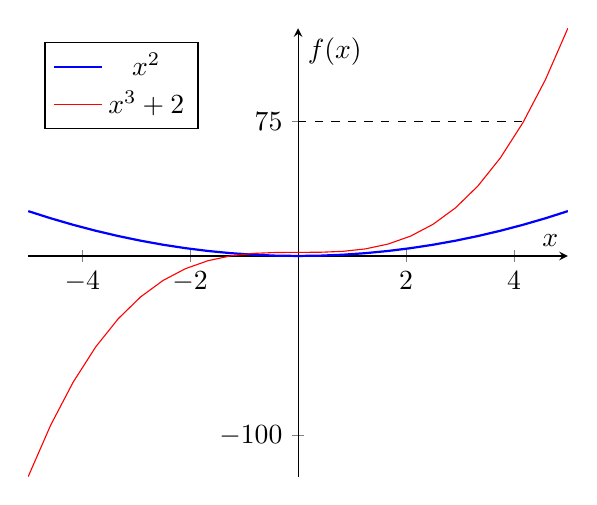
\begin{tikzpicture}
    \begin{axis} [
        xlabel=\(x\), ylabel=\(f(x)\),
        legend pos = north west,
        domain=-5:5, axis lines = center,
        ytick={-100,0,75}, 
    ]
        \addplot[blue, thick] {x^2};
        \addlegendentry{\(x^2\)}
        \addplot[red] {x^3+2};
        \addlegendentry{\(x^3+2\)}
        \addplot[dashed, domain=0:4.18] {75};
    \end{axis}
\end{tikzpicture}
\end{lstlisting}
\end{minipage}
\end{figure}

\verb|\addplot[dashed, domain=0:4.18] {75};| is particularly interesting because it goes against the general recommendation.
Here we are specifically creating an arbitrary dashed line at \verb|y=75| in the domain \verb|0:4.18|.

\paragraph{Note: }
Pay attention to the use of commas, colons and correctly creating a math environment.
Not using them correctly is a very common reason why your document won't compile.
\verb|\addplot{x^2};| has the expression written normally and ends with a colon (\verb|;|).
On the other hand, \verb|\addlegendentry{x^2}| is attempting to display \verb|x^2|, but without math mode \LaTeX\ doesn't know what to do --- hence the \verb|\(x^2\)|.

\subsection{Bar plot}

\begin{figure}[h]\centering
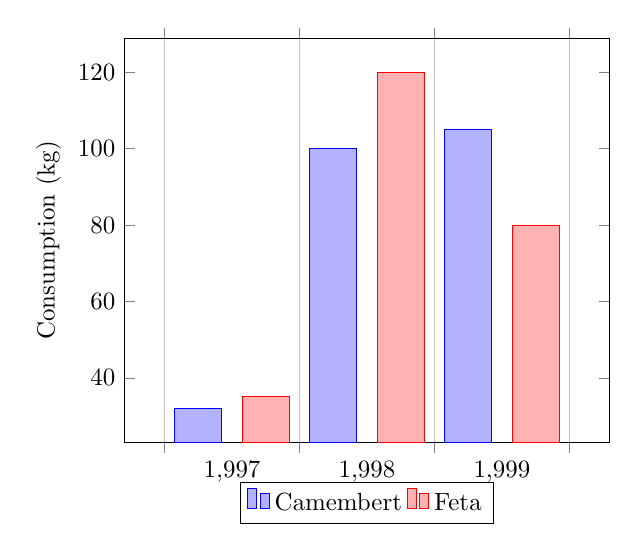
\begin{tikzpicture}[scale=0.9]
    \begin{axis}[
        ybar interval=0.7,
        ylabel=Consumption (kg),
        legend style={
            at={(0.5,-0.1)}, anchor=north,legend columns=-1
        },
    ]
    \addplot coordinates {
        (1997,32) (1998,100) (1999,105) (2000,58) 
    };
    \addplot coordinates {
        (1997,35) (1998,120) (1999,80) (2000,39) 
    };
    \legend{Camembert, Feta}
    \end{axis}
\end{tikzpicture}
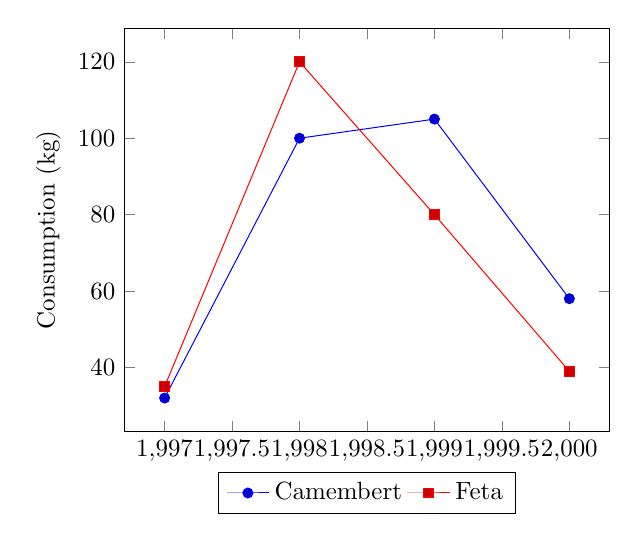
\begin{tikzpicture}[scale=0.9]
    \begin{axis}[
        ylabel=Consumption (kg),
        legend style={
            at={(0.5,-0.1)}, anchor=north,legend columns=-1
        },
    ]
    \addplot coordinates {
        (1997,32) (1998,100) (1999,105) (2000,58) 
    };
    \addplot coordinates {
        (1997,35) (1998,120) (1999,80) (2000,39) 
    };
    \legend{Camembert, Feta}
    \end{axis}
\end{tikzpicture}
\caption{A bar plot and the same data without \texttt{ybar}.}
\end{figure}

\begin{lstlisting}
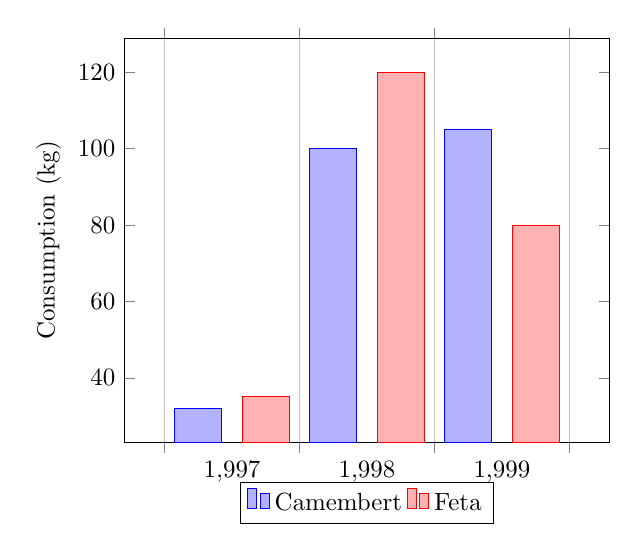
\begin{tikzpicture}[scale=0.9]
    \begin{axis}[
        ybar interval=0.7,
        ylabel=Consumption (kg),
        legend style={
            at={(0.5,-0.1)}, anchor=north,legend columns=-1
        },
    ]
        \addplot coordinates {
        (1997,32) (1998,100) (1999,105) (2000,58) 
        };
        \addplot coordinates {
            (1997,35) (1998,120) (1999,80) (2000,39) 
        };
        \legend{Camembert, Feta}
    \end{axis}
\end{tikzpicture}
\end{lstlisting}
The option \verb|ybar interval = 0.7| creates a bar plot in the y-direction with a bar thickness (in the x-direction) of 0.7.
On the right of it you can see the exact same plot without the \verb|ybar| option.
You may notice the data points in the year 2000 which are omitted --- this is also caused by \verb|interval|.
Play with it yourself, and take a look at the documentation examples for more customisation.

\verb|\legend style = {...}, | moves the legend from inside the plot box to the outside.
Notice that in the previous example we simply used \verb|legend pos|, but there is a lot that can be changed through styles.

This time around we created plots from coordinates, which are simply given as a list without commas, as highlighted below
The main use-case tends to be simple bar plots, because usually we would import data from a file, as in our next example.

\begin{lstlisting}
    \addplot coordinates {
        (x1,y1) (x2,y2) (x3,y3)...
    };
\end{lstlisting}

\paragraph{Challenge:}
Can you combine the two to create a graphical representation of a Riemann sum?
Below is one possible solution based on \href{https://tex.stackexchange.com/questions/197930/riemann-sum-with-pgfplots-cant-seem-to-make-graph-look-right}{this} thread in Stackexchange, an extremely important tool to finding solutions and learning!

\begin{figure}[h]\centering
\begin{minipage}{0.45\textwidth}
    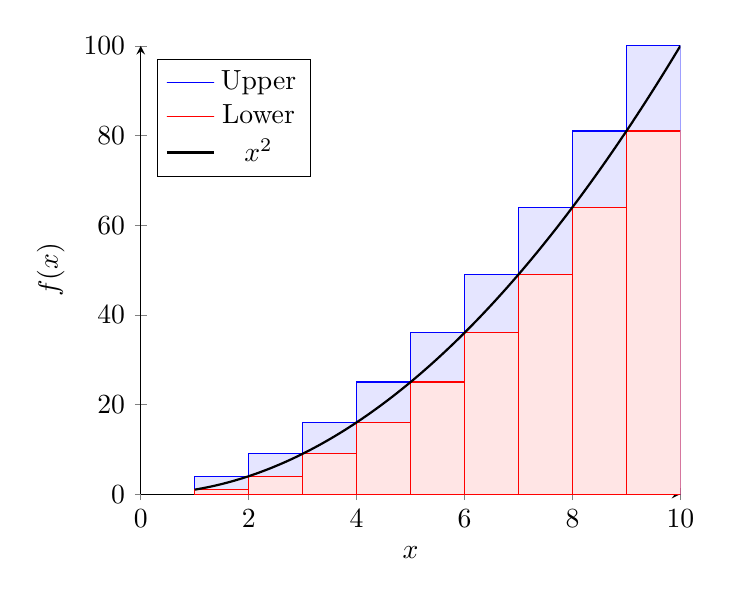
\begin{tikzpicture}
        \begin{axis}[xlabel= \( x \), ylabel= \( f(x) \),
                xmin=0, ymin=0, 
                axis lines = left, domain=0:10,
                legend pos = north west,
            ]
            \addplot [draw=blue, fill=blue!10, ybar interval, samples=10, domain=10:1]{x^2}\closedcycle;
            \addplot [draw=red, fill=red!10, ybar interval, samples=10, domain=1:10] {x^2}\closedcycle;
            \addplot[smooth, thick,domain=1:10,samples=40]{x^2};
            \legend{Upper, Lower, \( x^2 \) }
        \end{axis}
    \end{tikzpicture}
\end{minipage}
\hfill
\begin{minipage}{0.45\textwidth}
\begin{lstlisting}
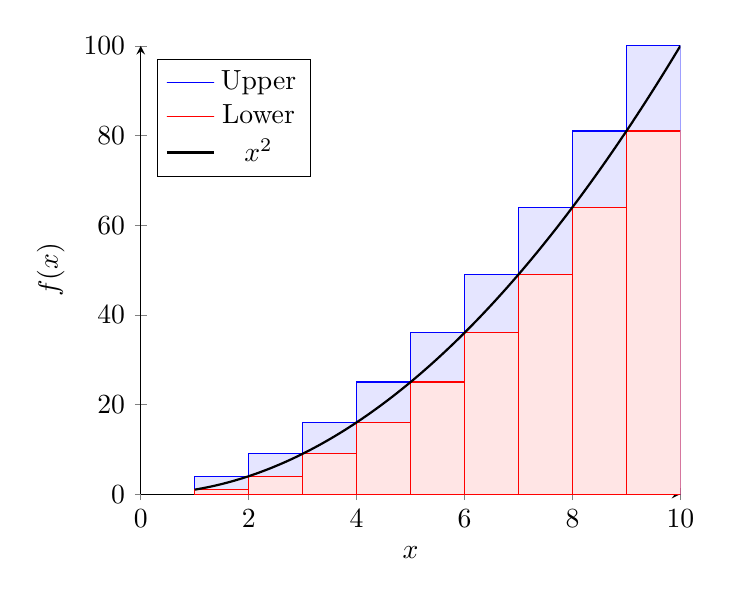
\begin{tikzpicture}
    \begin{axis}[xlabel= \(x\), ylabel= \(f(x)\),
            xmin=0, ymin=0, 
            axis lines = left, domain=0:10,
            legend pos = north west,
        ]
        \addplot [draw=blue, fill=blue!10, ybar interval, samples=10, domain=10:1]{x^2}\closedcycle;
        \addplot [draw=red, fill=red!10, ybar interval, samples=10, domain=1:10] {x^2}\closedcycle;
        \addplot[smooth, thick,domain=1:10,samples=40]{x^2};
        \legend{Upper, Lower, \( x^2 \) }
    \end{axis}
\end{tikzpicture}
\end{lstlisting}
\end{minipage}
\end{figure}

One important thing to note: the \texttt{draw} option controls the colour of the stroke/outline, while \texttt{fill} colours from the curve to the axis.
Now if you want to colour the area between two curves, you may want to look at section 5.7 of the documentation or work through an example, like \href{https://www.sqlpac.com/en/documents/latex-pgfplots-tikz-filling-areas-under-and-between-curves.html}{this} one.

By increasing the number of \texttt{samples} (subdivisions), we can even see that it approaches the integral.
\begin{figure}[h]\centering
    \begin{minipage}{0.45\textwidth}
        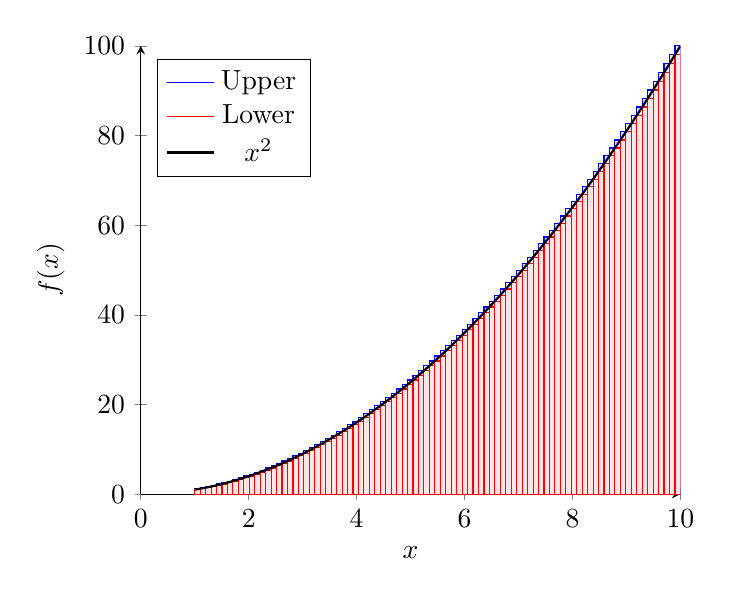
\begin{tikzpicture}
            \begin{axis}[xlabel= \( x \), ylabel= \( f(x) \),
                    xmin=0, ymin=0, 
                    axis lines = left, domain=0:10,
                    legend pos = north west,
                ]
                \addplot [draw=blue, fill=blue!10, ybar interval, samples=90, domain=10:1]{x^2}\closedcycle;
                \addplot [draw=red, fill=red!10, ybar interval, samples=90, domain=1:10] {x^2}\closedcycle;
                \addplot[smooth, thick,domain=1:10,samples=40]{x^2};
                \legend{Upper, Lower, \( x^2 \) }
            \end{axis}
        \end{tikzpicture}
    \end{minipage}
    \hfill
    \begin{minipage}{0.45\textwidth}
        \begin{lstlisting}
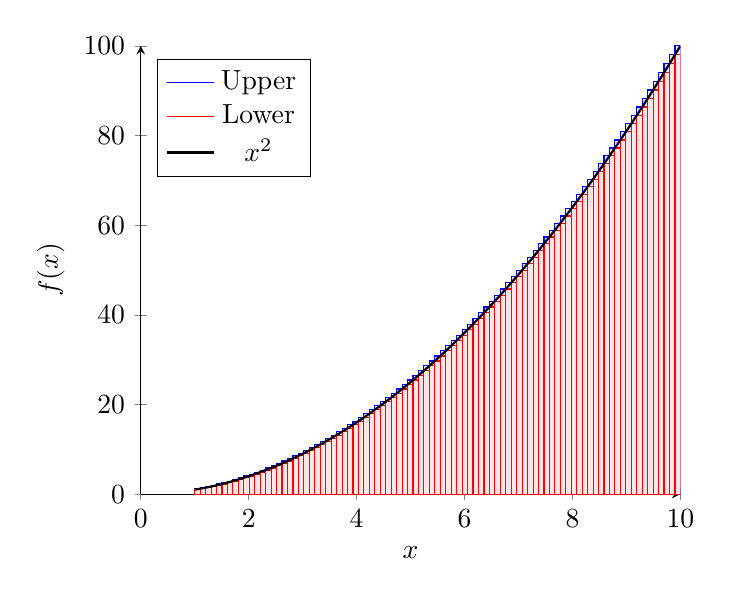
\begin{tikzpicture}
    \begin{axis}[xlabel= \(x\), ylabel= \(f(x)\),
            xmin=0, ymin=0, 
            axis lines = left, domain=0:10,
            legend pos = north west,
        ]
        \addplot [draw=blue, fill=blue!10, ybar interval, samples=90, domain=10:1]{x^2}\closedcycle;
        \addplot [draw=red, fill=red!10, ybar interval, samples=90, domain=1:10] {x^2}\closedcycle;
        \addplot[smooth, thick,domain=1:10,samples=40]{x^2};
        \legend{Upper, Lower, \( x^2 \) }
    \end{axis}
\end{tikzpicture}
        \end{lstlisting}
    \end{minipage}
\end{figure}

\subsection{Plot from data}
Data files are usually either \texttt{.csv} (with columns separated by commas), \texttt{.dat} or \texttt{.txt} (columns separated by tabs).
Generally if copying directly from LibreOffice/Excel, columns will be tab separated; whilst Octave/Matlab data by default is comma separated.

Three columns of random data were generated using LibreOffice and can be found in the examples folder called \texttt{data.dat}. They can also be seen below.
\lstinputlisting[caption={data.dat}]{Examples/data.dat}

\paragraph{Challenge:}
Can you import this data in to a table using \texttt{pgfplotstable}?
\textbf{Hint:} you may want to use these options: \verb|precision = 3| and \verb|fixed zerofill|.

\begin{figure}[h]\centering
\begin{minipage}{0.45\textwidth}
    \begin{tikzpicture}[scale=0.95]
        \begin{axis}[axis lines = left, ]
            \addplot [only marks] table {Examples/data.dat};
        \end{axis}
    \end{tikzpicture}
\end{minipage}
\hfill
\begin{minipage}{0.45\textwidth}
\begin{lstlisting}
\begin{tikzpicture}
\begin{axis}[axis lines = left]
    \addplot [only marks] table {Examples/data.dat};
\end{axis}
\end{tikzpicture}
\end{lstlisting}
\end{minipage}
\end{figure}

By default, it picks the first two columns to represent x and y.
In the next example, we deliberately choose the variables we want in each plot; allow automatic colouring \verb|\addplot+|; and combine a function with the data in the same axis.

It's worth noting that \texttt{pgfplots} tries to graph with the least amount of empty space, but we can always specify the minimum value of x and y in the axis with \verb|xmin| and \verb|ymin|.

\begin{figure}[h]\centering
\begin{minipage}{0.45\textwidth}
    \begin{tikzpicture}[scale=0.95]
        \begin{axis}[axis lines = left, ymin=0]
            \addplot+ [only marks] table[x=Var1, y=Var3] {Examples/data.dat};
            \addplot [dashed, domain=0:14] {10+3.5*x};
        \end{axis}
    \end{tikzpicture}
\end{minipage}
\hfill
\begin{minipage}{0.45\textwidth}
\begin{lstlisting}
\begin{tikzpicture}
\begin{axis}[ axis lines = left, ymin=0, ]
    \addplot+ [only marks] table[x=Var1, y=Var3] {Examples/data.dat};
    \addplot [dashed, domain=0:14] {10+3.5*x};
\end{axis}
\end{tikzpicture}
\end{lstlisting}
\end{minipage}
\end{figure}

\paragraph{Note:}
It is possible to get \texttt{pgfplots} to generate a linear regression from your data, but realistically we process the data elsewhere, and use this only for display.
If you would like to do it anyway, look at section 3.3 of the \texttt{pgfplots}' documentation \href{https://anorien.csc.warwick.ac.uk/mirrors/CTAN/graphics/pgf/contrib/pgfplots/doc/pgfplots.pdf}{here}.

\subsection{3d plots}
It is possible to do 3d plots with \texttt{pgfplots}, but beyond anything simple, you will find that using matlab and exporting the graph is far more computationally efficient\footnotemark.
Nevertheless, we will present a couple of examples here and go more in-depth with importing graphs in the following section.
\footnotetext{Alternatively, you may want to look into \href{http://tug.ctan.org/graphics/pgf/contrib/tikz-3dplot/tikz-3dplot_documentation.pdf}{\texttt{tikz-3dplot}}.}

Parametised plots are the simplest to get started, but pay attention to the use of \verb|x| in all directions.
Note that these examples are taken from \texttt{pgfplots}' documentation.
\begin{figure}[h]
\begin{minipage}{0.45\textwidth}
    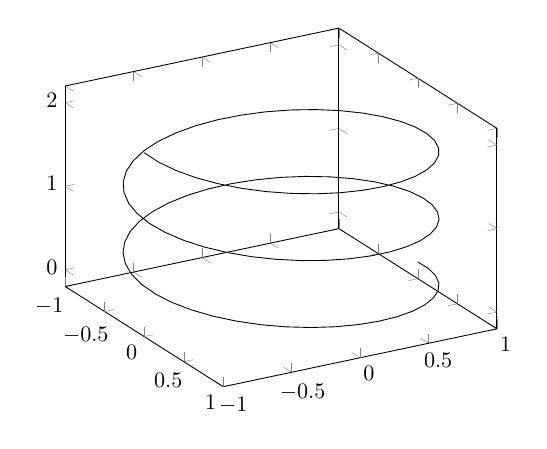
\begin{tikzpicture}[scale=0.8]
        \begin{axis}[view={60}{30}]
            \addplot3 [domain=0:5*pi,samples=100,samples y=1,]
            (
                {sin(deg(x))}, {cos(deg(x))}, {2*x/(5*pi)}
            );
        \end{axis}
    \end{tikzpicture}
\end{minipage}
\hfill
\begin{minipage}{0.45\textwidth}
\begin{lstlisting}
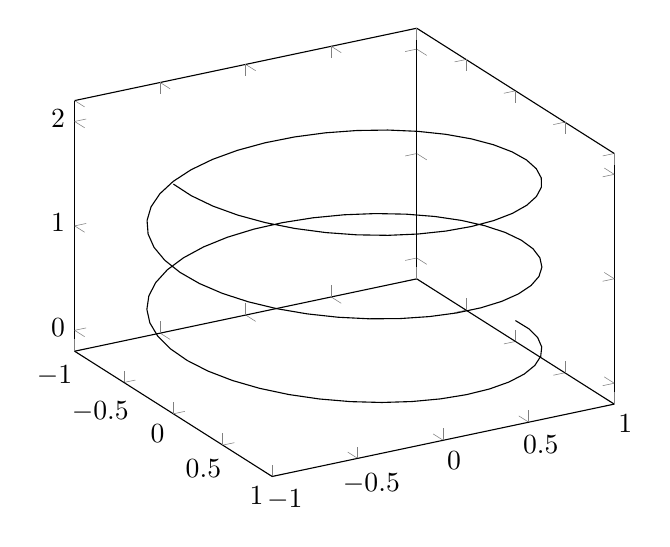
\begin{tikzpicture}
    \begin{axis}[view={60}{30}]
        \addplot3 [domain=0:5*pi,samples=100,samples y=1,]
        (
            {sin(deg(x))}, {cos(deg(x))}, {2*x/(5*pi)}
        );
    \end{axis}
\end{tikzpicture}
\end{lstlisting}
\end{minipage}
\end{figure}

\begin{figure}[h]
\begin{minipage}{0.45\textwidth}
    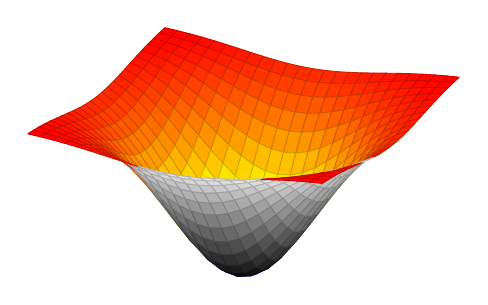
\begin{tikzpicture}[scale=0.8]
        \begin{axis}[hide axis,xlabel=$x$,ylabel=$y$,mesh/interior colormap name=hot,colormap/blackwhite,]
            \addplot3 [  domain=-1.5:1.5,surf]{-exp(-x^2-y^2)};
        \end{axis}
    \end{tikzpicture}
\end{minipage}
\hfill
\begin{minipage}{0.45\textwidth}
\begin{lstlisting}
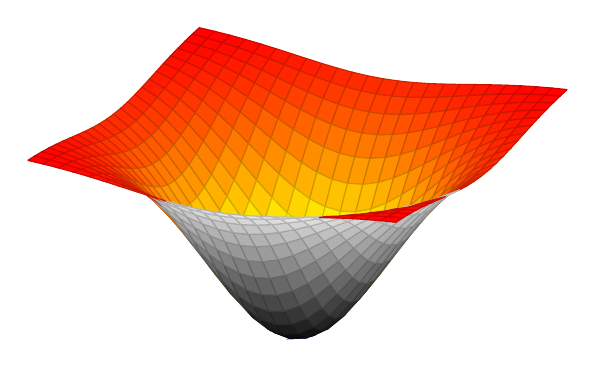
\begin{tikzpicture}
    \begin{axis}[hide axis,mesh/interior colormap name=hot,colormap/blackwhite,]
        \addplot3 [domain=-1.5:1.5,surf] {-exp(-x^2-y^2)};
    \end{axis}
\end{tikzpicture}
\end{lstlisting}
\end{minipage}
\end{figure}